\chapter{Investigation of Visualization Tools Using a Feature Classification Scheme}
\label{chap:Tools}

In this section we analyze selected visualization tools and their ability to visualize large time-oriented data. The implementation of each success criterion in chapter \ref{chap:scalability} was analyzed, resulting in ranking of the various tools that were considered. For database metrics row limitations were compared and for analytical, visualization and interaction techniques a classification scheme was developed. \\*

\section{Selection of Tools}\label{tool:selection}
The tools in this section were selected based on their relevance in business. In the era of self-service data science, business user expect tools to be both easy to use and to be complete. Ease-of-use is achieved by a graphical user interface  (\gls{GUI}), the need for little prior programming skills and the tool's universal use in many application areas. At the same time tools could be regarded as "complete" if they offer all relevant functions needed to support the analyst in the user tasks. Consequently, the choice of a visualization tool or framework is a balance between ease-of-use and completeness. According to ITCentralStation and the Magic Quadrant for Business Intelligence and Analytics Platforms 2017  \cite{ITCentralStation2017, Sallam2017} Qlik, Tableau and Microsoft are the leading visionaries among BI Vendors. All of these tools claim to support the user in data visualization, self-service data science and to be easy to use - making Qlik, Tableau and Microsoft Power BI popular visualization tools  (\ref{tools}). Their strength lies in the user support and their universality. Nevertheless, each tool is fee-based, which results in investment costs. \\
Commercial software tends to take more time than open-source software when developing and integrating advanced visualizations for large data  \cite{Zhang2012, Simon2014}. Therefore, we added an open-source visualization framwork to our selection: d3.js is a well-known choice for visualization in the visualization community, as it is a free open-source JavaScript library and offers a wide range of visualization possibilities.
Thus, the selection of tools are Qlik Sense, Tableau, Microsoft Power Bi and d3.js. The system requirements are listed in table \ref{tab:tool:system}.

\begin{table}[H]
    \centering
    \begin{tabular}{l l l l l l l l l}
        Tool & System Requirements & Costs & Open-Source & GUI\\
        \hline
        \rowcolor{lightblue}Power BI & >= Windows 7  & free/commercial & x & \checkmark\\
        Qlik Sense & >= Windows 7  & free/commercial & x & \checkmark\\
        \rowcolor{lightblue}Tableau & >=Windows 7; >= OSX 10.10 & commercial & x & \checkmark\\
        d3.js & Browser  & free & \checkmark  & x
    \end{tabular}
    \caption{Tool Requirements}
    \label{tab:tool:system}
\end{table}

%Nevertheless, market relevance reports from research and advisory companies such as Gartner, Forrester, Barc usually do not publish detailed scoring models.  Thus, the ranking might not be appropriate to our needs.


% \iffalse
% ADV in business context requires software that is able to scale visualization in an "effective manner" \cite{Russom2011}. Offering ADV techniques, parameterization, interaction and analytical methods such as data abstraction \cite{Tegarden1999,Aigner2011,Eick2002,Zhang2012} are core functions of ADV software. \\*
% \textbf{The Role of APIs}
% Commercial software tends to need more time for the development and integration of advanced visualization for large data \cite{Zhang2012, Simon2014}. To bridge the gap, vendors started to offer a bunch of APIs to expand the visualization functions. 
% % data load for BigData: 
% \textbf{Software not included in this work}
% As the goal of this work is to compare visualization tools in business we only consider software which is 
% \begin{enumerate}
%     \item generic: not specialized to one domain
%     \item integrates visualization features
% \end{enumerate}

% Furthermore, the software needs visualization features, the ability to present time-dependent data. Software with one of the following items is intentionally not considered: 
% \begin{enumerate}
%     \item Software that only presents one-dimensional data. 
%     \item Software that is specialized to data mining.
% \end{enumerate}
% \fi


\section{Visual Scalability of Visualization Tools}\label{tool:scalability}
The selected tools are evaluated against the criteria discussed in section \ref{success} based on studying each tool's documentation \cite{Qlik2017, Tableau2003, BI2017, Bostock2012} as well as by actively using the tools. 
\label{tool:classification}

The basis of assessment with respect to \textit{visualization, analytical and interaction characteristics} is a classification scheme based on the success criteria of section \ref{success}. These aspects are assessed on the two business relevant scales for self-service tools: the criterion of completeness  (table \ref{table:completeness}) and the criterion of required programming skills  (table \ref{table:programming-skills}). The factor \textit{completeness} serves as an indicator of how many features of the defined criteria the business can user achieve with this tool. As an example, completeness in aggregation metaphors displays how many visualization techniques include aggregation metaphors. Because completeness is difficult to measure we decided to perform a \textit{relative} comparison of completeness.

\begin{table}[H]
\centering
	\caption[Criterion Completeness]{Criteria Completeness: extend to which success criterion is implemented in tool}
	\label{table:completeness}
	\begin{tabu}{cl}
	\hline
	Points & Criteria\\
	\hline
	0 & Not existing\\
	1 & partially implemented \\
	2 & fully implemented \\
	\hline
	\end{tabu}
\end{table}

The consideration of programming skills in business is important as the standard business user may have little programming knowledge  (compare \ref{tasks}). Moreover, programming skills are associated with investment costs. The higher the required programming skills the higher the investment costs are. Programming skills are measured by the user knowledge required to achieve a feature. The most complex level is when a feature can only be implemented by a tool-specific programming language  (1). On the next level, programming knowledge is required but in a popular programming language  (2). Popular programming languages such as R, Java, JavaScript, python and C can be used in other environments, which increases the probability that the user knows the language. The next step is to embed a feature via drag and drop  (3). Least effort is needed when the tool offers the feature automatically  (4). The difference from level 2 to level 3 is much larger than the difference from level 3 to level 4. Thus, the ranking is not linear but ordinal. We assume that a tool-specific language requires additional training effort. 
\begin{table}[H]
	\centering
	\caption[Criterion Programming-Skills]{Criteria Required Programming-Skills to use the assessed aspect}
	\label{table:programming-skills}
	\begin{tabu}{cl}
	\toprule
	Points & Criteria\\
	\midrule
	1 & Feature can be programmed, but in a tool-specific programming language\\
	2 & Feature can be programmed in a popular programming language  (R,JavaScript,Java)\\
	3 & Available by drag and drop \\
	4 & Automatic support by tool\\
	\bottomrule
	\end{tabu}
\end{table}

All ten success criteria rated for completeness and programming skills have been combined in the tool criteria score  (\gls{TCS}). Each feature of the tool has been assigned a tuple consisting of  (Programming Skills, Completeness). If the assessed aspect did not exist, 0 was assigned.
Based on the assessment of different features  we draw our conclusion  (\ref{conclusion}).
% \iffalse
% \subsection*{R}
% \textbf{Analytical Techniques}\\
% Out of the five tools R has the most extensive offer of analytical methods for time-series data. It is possible to detect patterns such as outliers with tsoutliers \cite{Chen1993} and clusters with tsclust \cite{Manso2015}, do advanced analytics with tswge \cite{tswge} and forecasting with zra \cite{zra}.
% \textbf{Visualization Techniques}\\
% R supports standard visualization such as histograms, line charts and scatter plots. Advanced visualization techniques for large data sets 
% \textbf{Aggregation}\\*
% In the maps-package R offers the possibility to adjust the resolution with the parameter resolution. Resolution 0 maps the whole database whereas a higher resolution collapes data points within the resolution to one single point. This option allows to aggregate data and to only show the perceptual important points  (PIP).
% The bigvis and the hexbin package implement binning to condense large data sets \cite{Wickham2013}.
% \textbf{Pixel-oriented} Time Series are visualized with mvtsplot \cite{mvtsplot}. This package allows to compare multivariate time-series data.
% \textbf{Interaction Techniques}\\
% Plot\_ly () \cite{plotly} supports a brushing function with drill-down.
% Shiny supports panning and zooming as well as linking and brushing.
% Linked views are supported by plot\_ly () with and without shiny. 
% Fish-eye views are implemented in the fisheyeR () package. 
% The time range can be decreased by limiting the data range inside the code.
% Animation can be achieved by using plot\_ly () and ggploty (). Moreover, plot\_ly () offers linked animated views.
% \textit{Dygraphs} includes also navigational sliders called Range Selector, panning and zooming and brushing of data items.
% \fi


\subsection{Qlik Sense}\label{tool:QS}
Qlik Sense is the self-service product of Qlik. Qlik was founded in 1993 with the goal to "mimic how the brain works".  \cite{Qlik2017}. They offer five products QlikSense (QS), \gls{QS}   Cloud, QlikView (QV), QlikView NPrinting, Qlik DataMarket and the Qlik Analytics platform. \gls{QS}   1.0 was released in September 2014 for visual analytics. 
\par
\textbf{Database Metrics}\\
QS inherits the data load limitations of QlikView: A \gls{QS}   document cannot have more than 2,147,483,648 distinct values in one field. This limitation still allows Qlik for handling large and huge data sets according to our definition. In context of visualization QS limits the initial fetch to 10.000 but gives the opportunity to fetch more data if needed.
\par
\textbf{Analytical Techniques}\\
QS integrates methods to reduce data size. For this the tool specific \href{https://help.qlik.com/en-US/sense/3.2/Subsystems/Hub/Content/ChartFunctions/SetAnalysis/set-analysis-expressions.htm}{set expressions  (\gls{SE})} are often required. Set expressions are a Qlik-specific language based on the signs \{,(,<,=,\$ to define a set of values. \\
\textbf{Example:}\\
The set expression \{\$<Year=\{2009\}>\}  can be interpreted as "All data items of the current selection in the year of 2009".\par
Horizontal data reduction is implemented in the \gls{QS} feature called  \href{https://help.qlik.com/en-US/sense/3.2/Content/Videos/Videos-dimensions-limitations.htm}{\textit{Dimension Limitations}}. With dimension limitation the user can set the number of dimensions in the \gls{GUI}-panel by applying conditions to the columns (For the data model of rows and columns refer to \ref{data}.). 
Dimensions are aggregated with \href{https://help.qlik.com/en-US/sense/3.2/Subsystems/Hub/Content/Dimensions/calculated-dimensions.htm}{\textit{calculated dimensions} (\gls{CF})}, meaning that one or more dimensions are combined and saved as a new dimension by using \gls{SE}.
Data reduction is part of \gls{QS}   Server. With \href{https://help.qlik.com/en-US/sense/2.1/Subsystems/Hub/Content/Scripting/Security/dynamic-data-reduction.htm}{\textit{dynamic data reduction  (\gls{DDR})}} rows can be hidden for a group of users. Data rows can be reduced using an SQL-like scripting language inside the backend. Internally, QVD files compress data. Thus, the data size is decreased. 
At the frontend, the user can apply \href{https://help.qlik.com/en-US/sense/2.1/Subsystems/Hub/Content/Visualizations/FilterPane/filter-pane.htm}{\textit{filters}}.
Data clustering in \gls{QS}   is implemented by \href{https://help.qlik.com/en-US/sense/3.2/Subsystems/Hub/Content/Scripting/AggregationFunctions/aggregation-functions.htm}{\textit{aggregation functions}}. These use \gls{SE} and range from basic  (min, avg, max) to advanced statistical functions (linear regression, correlation). With these aggregation functions \gls{QS}   offers some analytical methods. However, \gls{QS}   has no integration to an analytical program.
\par

\textbf{Visualization Techniques}\\
QS offers \href{https://help.qlik.com/en-US/sense/2.1/Subsystems/Hub/Content/Visualizations/visualizations.htm}{eight built-in visualization techniques}\footnote{The chart types are bar charts, line charts, pie charts, scatter plots, treemap, maps, combi charts and gauge charts.}. If an additional technique is wanted, the user can either install one of the community's self-made extensions or build his own \href{https://help.qlik.com/en-US/sense-developer/3.2/Subsystems/Extensions/Content/extensions-getting-started.htm}{\textit{visualization extension}} with JavaScript and QEXT files. \gls{QS}   provides an extension template which supports the user in writing his extensions. Moreover, Qlik provides 20 high-level-APIs that supports the user in writing a custom extension. However, the user needs to know JavaScript, html  , as well as \gls{QS}'   own QEXT-language. \\*
From the \gls{QS} standard repertoire none of the visualization techniques correspond to the studied visualization techniques of chapter \ref{chap:scalability}. With d3.js it would be possible to build these visualization techniques and integrate them in \gls{QS}. With JavaScript visualizations with multi-resolution and aggregation markers can also be embedded in \gls{QS}. However, these advanced metaphors have to be implemented for each technique and thus are only available for some techniques. Moreover, the implementation requires coding-skills. 

Advanced visual metaphors are supported by \gls{QS} for one chart type: the scatter plot, where large data is aggregated by aggregation markers. When the scatter plot is shown at an overview level accumulated data points are represented by squares as in figure \ref{fig:smartdatacompression} and \ref{fig:dense}. Data density is mapped to the color attribute.  The darker the square the denser the data. Since data is sparse at detail level, the squares change to points (figure \ref{fig:sparse}). The so-called \href{https://help.qlik.com/en-US/sense/2.1/Subsystems/Hub/Content/Visualizations/scatter plot/scatter-plot.htm}{\textit{Smart Data Compression} (\gls{SDC})} is one implementation for the aggregation of large data amounts. However, \gls{SDC} is only available for one technique. For this reason \gls{QS} still lags behind the present day requirements.


\begin{figure}[H]
    \centering
    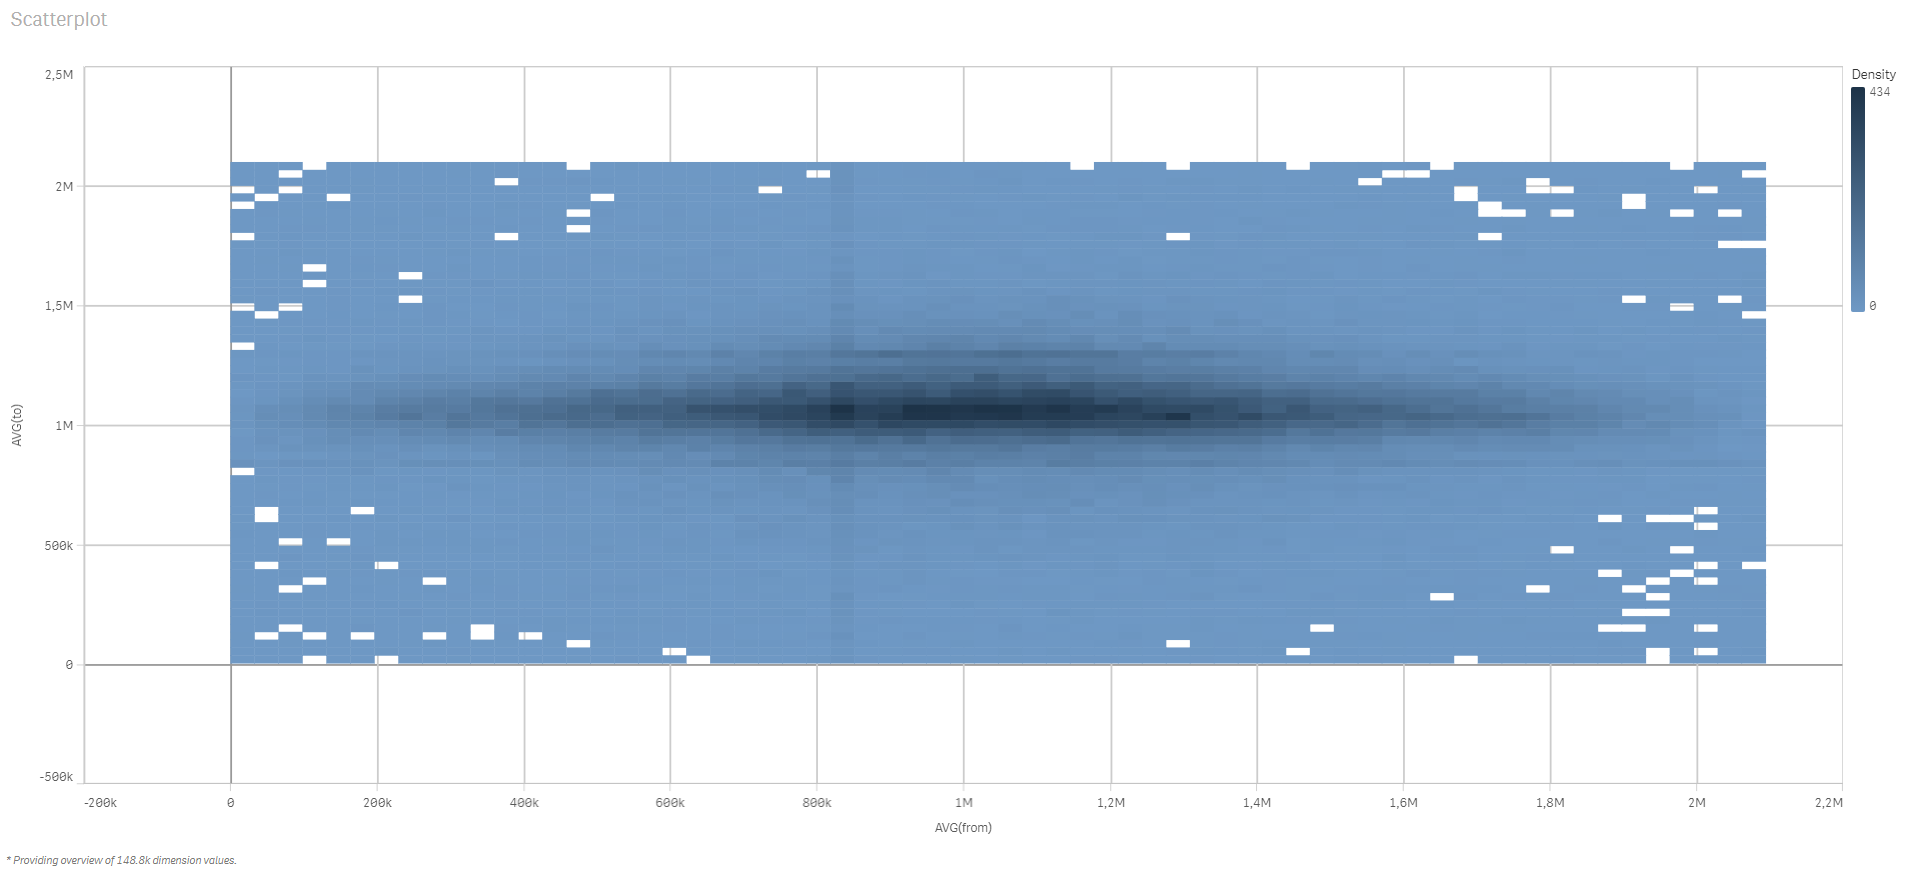
\includegraphics[width=10cm]{src/images/SmartDataCompression}
    \caption[Smart Data Compression: Overview]{Smart Data Compression: Overview level which shows aggregated data points by squares and color and changes the shape if zoomed in.}
    \label{fig:smartdatacompression}
\end{figure}

\begin{figure}[H]
    \centering
    \subfloat[Sparse Area]{\label{fig:sparse}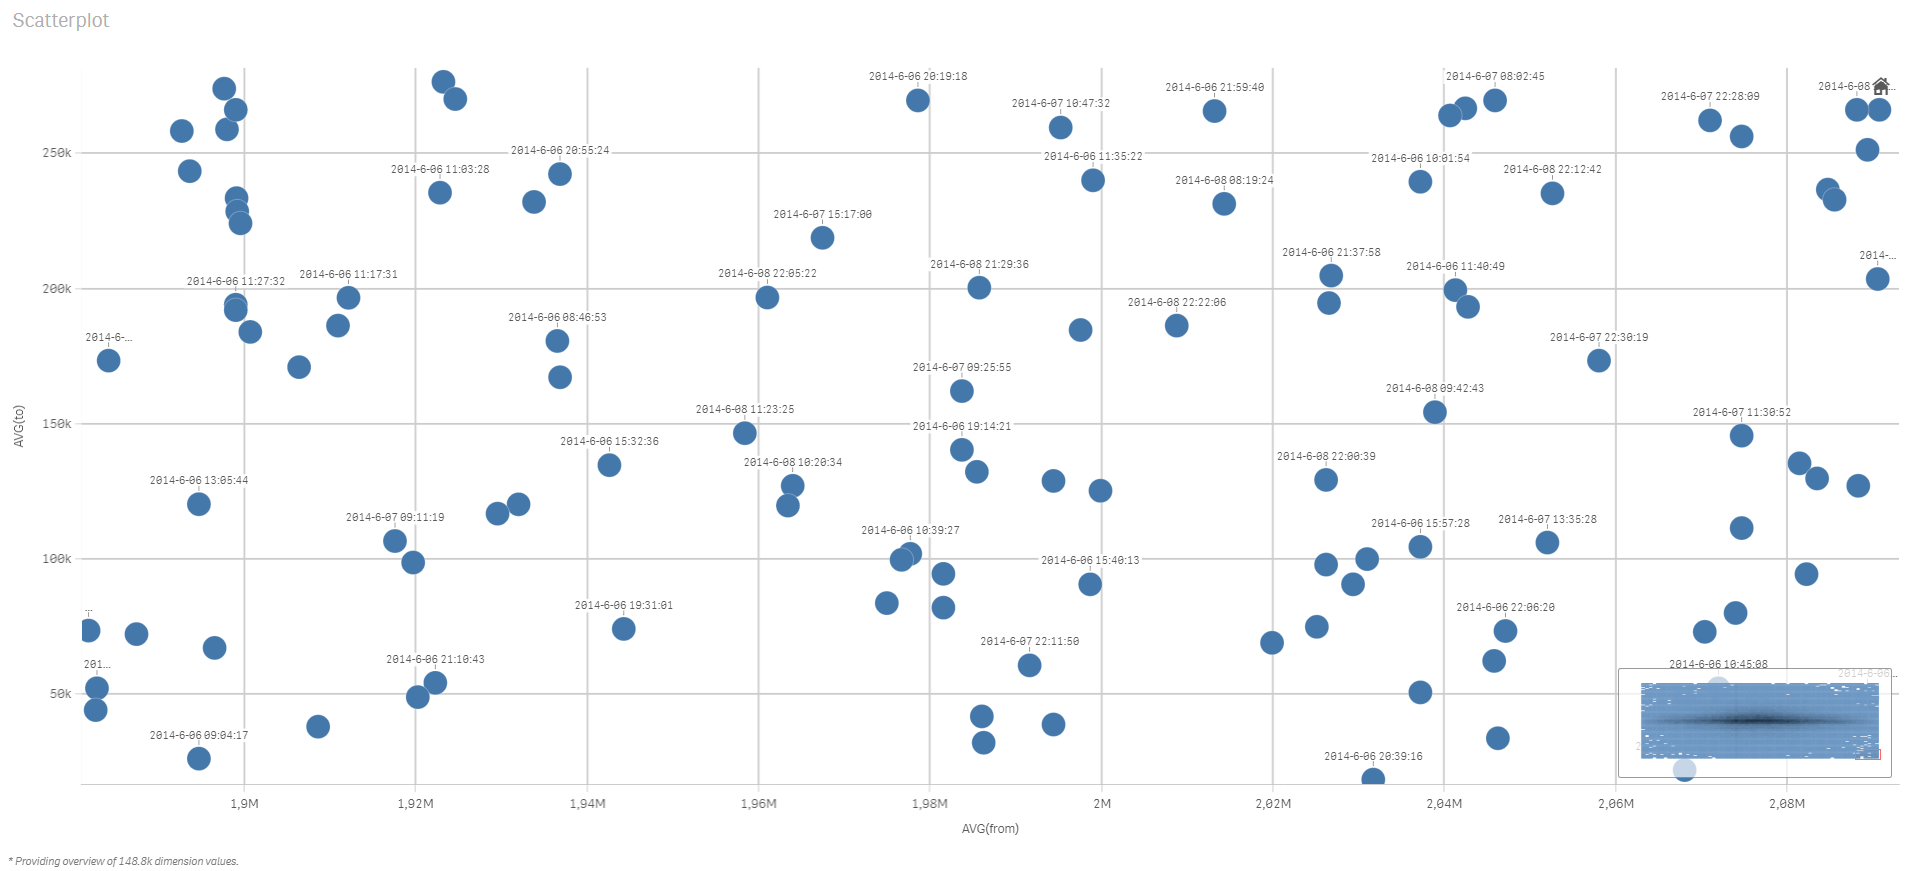
\includegraphics[width=10cm]{src/images/SmartDataCompressionI}}
    \qquad
    \subfloat[Dense Area]{\label{fig:dense}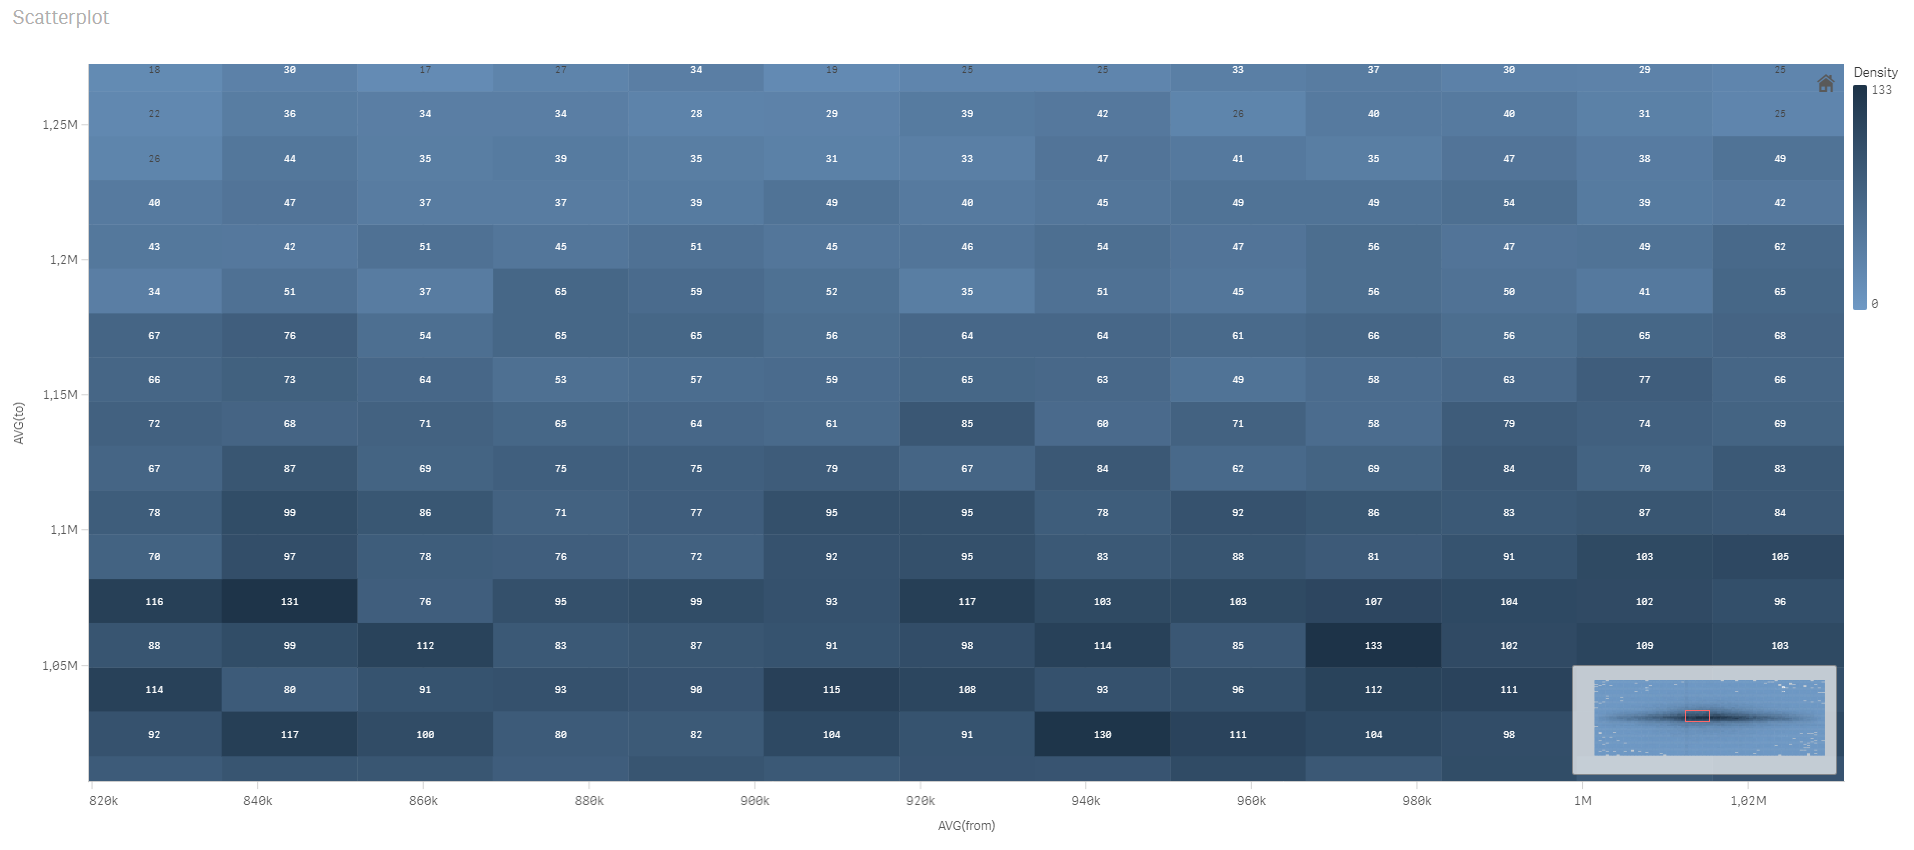
\includegraphics[width=10cm]{src/images/SmartDataCompressionII}}
    \caption[Smart Data Compression: Detail]{Smart Data Compression: Detail level with point markers (\ref{fig:sparse}) and numbered squares (\ref{fig:dense}).}
    \label{fig:smartdatacompression2}
\end{figure}

\textbf{Interaction Techniques}\\
In terms of interaction techniques \gls{QS}   offers drill-down and navigation techniques. Zooming and filtering are possible for all visualizations. If the zoom is active, mini charts  (\gls{MiC}) appear that are one implementation of navigational maps. Mini Charts come as a navigational slider in which a miniature version of the whole data set is shown. In figure \ref{fig:smartdatacompression} and figure \ref{fig:smartdatacompression2} \gls{MiC} appear in the right lower corner.
Filters can be applied by making selections or dragging a filter inside the visualization. With multiple linked views all views are then adapted to the current selection. Thus, \gls{QS}   offers brushing-and-linking. For details the user can search \gls{QS}   with \href{https://help.qlik.com/en-US/sense/2.1/Content/Videos/Videos-global-smart-search.htm}{\textit{Smart Search}} in which the dimensions, measures and metadata is searched and visualizations, tables and KPIs are displayed. Distortion techniques are not offered but can be implemented with extensions. 
\pagebreak
\subsection{Tableau}\label{tool:Tableau}
Tableau was founded in 2003 as a spinoff from  a university project. Tableau offers three main products: Tableau Desktop, Tableau Public and Tableau Server.
\par
\textbf{Database Metrics}\\
Tableau has no limitations for the data load.
\par
\textbf{Analytical Techniques}\\
Tableau's strength is its easy-to-use analytical functions. On one hand, Tableau offers built-in modelling functions that can be activated via drag and drop: prediction, trend line, cluster, average and median. On the other hand data reduction is supported. Horizontal and vertical reduction is implemented by \href{http://onlinehelp.tableau.com/current/pro/desktop/en-us/extracting_data.html}{\textit{Data Extracts  (\gls{DEx})}}. Data extracts can be built based on a data connection and then reduced by limiting the data that is loaded. Dimensions can be reduced by hiding columns while creating \gls{DEx}. Only visible columns are then loaded into the dashboard. Dimensions are aggregated in a similar manner to how it is done with \gls{QS}, i.e. by using \href{http://onlinehelp.tableau.com/current/pro/desktop/en-us/calculations_calculatedfields.html}{\textit{calculated fields} (\gls{CF})}. Moreover  \href{http://onlinehelp.tableau.com/current/pro/desktop/en-us/calculations_calculatedfields_aggregate.html}{\textit{aggregated calculations}} reduce data vertically by clustering them. Another implementation of vertical data reduction is the use of  \href{http://kb.tableau.com/articles/howto/adding-filters-to-dashboards}{\textit{filters}} that can be added in the frontend. Tableau's analytical capabilities can be enhanced by loading R scripts into Tableau. R offers additional data reduction capabilities such as \gls{PCA} or \gls{SOM}.
\par
\textbf{Visualization Techniques}\\
Tableau offers 22 built-in visualization techniques such as heat maps or scatter plots \cite{Tableau2003} \footnote{Tableau's chart types are heat maps, symbol maps, stacked bars, pie charts, horizontal bars, side-by-side bars, treemaps, circle views, side-by-side circles, continuous lines, discrete lines, dual lines, area charts,  discrete area charts, dual combination, scatter plots, histogram, box-and-whisker plots, Gantt chart, bullet graphs and packed bubbles.}.
Visualization extensions are not possible even though Tableau has a \href{https://www.google.de/search?client=safari&rls=en&q=tableau+javascript+api&ie=UTF-8&oe=UTF-8&gfe_rd=cr&ei=2oLOWKveK5LZ8AeXl4bIBw}{JavaScript API}. This API allows for the integration of a Tableau dashboard into a web page, but is not built for writing JavaScript extensions for Tableau. In addition, advanced metaphors such as multi-resolution, data abstraction or aggregation markers are not supported. 
In sum, Tableau is a well-known choice in the visualization community but it does not support large scale visualization features. 
\par

\textbf{Interaction Techniques}\\
In terms of drill-down techniques, Tableau offers automatic zooming and  \hyperlink{http://kb.tableau.com/articles/howto/adding-filters-to-dashboards}{filtering}. The \textit{focus mode} expands one visualization to full screen and thus, allows the user for having a detailed view on the visualization. 
Regarding navigation techniques Tableau integrates \href{https://www.tableau.com/de-de/whitepapers/enhancing-visual-analysis-linking-multiple-views-data}{\textit{multiple linked views}}.
Distortion techniques, search and navigational sliders are not supported. 
\par
\pagebreak
\subsection{Power BI}\label{tool:PowerBI}
Microsoft Power BI first appeared in September 2013. It is divided into three services: Power BI Mobile, Power BI Desktop and Power BI service. Power BI Mobile allows reports for being accessed by a portable device. Power BI Desktop is a business analytics suite for creating visualizations and reports and Power BI service publishes reports. We are concentrating on Power BI Desktop.
\par
\textbf{Database Metrics}\\
Power BI has no limitations for the data load.
\par
\textbf{Analytical Techniques}\\
Data reduction in Power BI is implemented in a similar manner to \gls{QS}   and Tableau. Dimensions can be aggregated with 
horizontal data reduction implemented by  \href{https://powerbi.microsoft.com/en-us/documentation/powerbi-desktop-tutorial-create-calculated-columns/}{\textit{calculated columns} (\gls{CF})}. Vertically, data can be reduced both in the frontend and in the backend. With \href{https://community.powerbi.com/t5/Desktop/How-to-reduce-the-amount-of-data-that-is-loaded-into-my-Power-BI/td-p/54112}{\textit{views}} on the database  (V) and joins, data extracts are created. Joins and Views use SQL. Moreover, data sets can be extracted  (\gls{DEx}) from within the \gls{GUI} with \href{https://Power BI.microsoft.com/de-de/blog/power-bi-desktop-october-feature-summary/#grouping}{\textit{Inclusion/Exclusion}} of data points. Moreover, \href{https://powerbi.microsoft.com/en-us/documentation/powerbi-service-add-a-filter-to-a-report/}{\textit{filters}} can be added and  \href{https://powerbi.microsoft.com/en-us/documentation/powerbi-service-aggregates/}{\textit{aggregates}} built.
Besides the own core functions for data reduction Power BI is connected to analytical programs such as \href{https://Power BI.microsoft.com/de-de/blog/power-bi-desktop-october-feature-summary/#grouping}{\textit{R, Mixpanel or comScore.}}
\par

\textbf{Visualization Techniques}\\
Microsoft Power BI offers eight built-in \href{https://powerbi.microsoft.com/en-us/documentation/powerbi-service-visualization-types-for-reports-and-q-and-a/}{\textit{visualization techniques}}, 15 available techniques at the MarketPlace and 75 visualization apps in the visuals gallery. Additionally, the user can build custom visualization apps by writing \href{https://powerbi.microsoft.com/en-us/documentation/powerbi-custom-visuals-getting-started-with-developer-tools/}{\textit{TypeScript}} or \href{https://powerbi.microsoft.com/en-us/guided-learning/powerbi-learning-3-11h-r-visual-integration/}{\textit{R}} functions. Out of the 98 techniques none of them implements any discussed techniques of chapter \ref{chap:scalability}. So far, advanced metaphors are not supported. One approach to aggregation markers are \hyperlink{https://Power BI.microsoft.com/de-de/blog/power-bi-desktop-october-feature-summary/\#grouping}{\textit{Groups}} that can be combined with drill-down options.
\par

\textbf{Interaction Techniques}\\
Power BI embeds zoom and filter functions. Similar to Tableau, Power BI also offers a focus mode. Thus, Power BI implements an overview-and-detail view. 
With \href{https://powerbi.microsoft.com/en-us/documentation/powerbi-service-about-filters-and-highlighting-in-reports/}{\textit{highlighting}} Power BI includes brushing-and-linking. Therefore, the user can control which windows are connected. The app \textit{Advanced Time Slicer} is one implementation of the "navigational map" technique for time-oriented data. However, navigational maps are only implemented for one visualization technique. Navigation in Power BI is also realized by the search mechanism Power \gls{Q+A} that answers \gls{NLP}-questions regarding the data set. Power  \gls{Q+A}  includes filtering with the keywords WHERE, AFTER, BEFORE, BETWEEN, WITH or by naming the date. Distortion techniques are not supported. They can be embedded with visualization extensions  (\gls{E}) written in TypeScript.

\pagebreak
\subsection{d3.js}\label{tool:d3.js}

d3.js is a JavaScript library used for visualization. It binds input data to existing web elements of the Document Object Model (\gls{DOM}) and visualizes data based on SVG, HTML5 and CSS. The resulting chart is the document. Data Handling is managed by the underlying data source. Data modeling can be handled by other JavaScript libraries such as node.js.
\par
\textbf{Database Metrics}\\
d3.js has no limitations for the data load.
\par
\textbf{Analytical Techniques}\\
While d3.js is only designed to visualize data it does not inherently offer analytical techniques. Therefore, a number of JavaScript libraries  (\gls{L}) exist that can be combined with d3.js. Some examples are simplestatistics.js, regression.js, node.js with the packages data-reduction, ml-pca or dimensionality-reduction. Since JavaScript allows for the integration of libraries there is no limit to analytical functions. Thus, d3.js does not offer any data reduction techniques automatically. 
With respect to data abstraction, JavaScript libraries offer abstraction functions for the frontend. Some examples are d3.hexbin that allows for binning, simplify.js for data abstraction or clusterfck.js for clustering. Simplify.js for example reduces data points on polylines while maintaining the characteristic shape of the polyline. Besides libraries d3.js can be used together with any REST API compatible backend and the data reduction abilities then depend on the backend.
\par

\textbf{Visualization Techniques}\\
By writing JavaScript code any visualization technique and any advanced metaphor can be implemented. Currently, various implementations are \href{https://github.com/d3/d3/wiki/Gallery}{available} that help the user to create his own visualizations. For aggregation metaphors \href{http://bl.ocks.org/gisminister/10001728}{\textit{marker clustering}} is one example. Moreover, tutorials exist that describe how marker clustering can be implemented with  \href{https://www.phase2technology.com/blog/using-d3-quadtrees-to-power-an-interactive-map-for-bonnier-corporation/}{quadtrees}  \cite{Morrison2014}.
\par

\textbf{Interaction Techniques}\\
d3.js allows for the integration of various interaction techniques such as Zooming, Filtering or Brushing-and-Linking. Distortion techniques can be achieved with the plugin \hyperlink{https://bost.ocks.org/mike/fisheye/}{\textit{Fisheye Distortion  ( \gls{FD}  )}}  \cite{Bostock2012} which allows for circular, linear and logarithmic distortion.
Perspective walls can be implemented with \hyperlink{https://bl.ocks.org/mbostock/10571478}{\textit{Perspective Transformation  (PT) }}  \cite{Bostock2017}.\\

\pagebreak
\section{Results}
In this section the tools' visual scalability is compared with regard to the aspects \textit{database metrics, analytical, visualization and interaction techniques}. Tools are ranked according to the extent to which they implement each respective aspect.

\subsection{Tool ranking for database metrics}
As \gls{QS} is the only tool which restricts data loads both at the backend and the frontend \gls{QS} is outperformed by Tableau, Power BI and d3.js which is shown in \ref{table:databasemetrics}. The tools are ranked from one to four. Rank one offers no limitations while rank four offers most limitations in database metrics.
% Ranking for Database Metrics
\begin{table}[H]

    \begin{tabular}{|l| l l l l l|}
        \hline
        \multicolumn{2}{|c}{}   & d3.js  & \gls{QS}    & Power BI & Tableau\\\hline
        \multirow{2}*{Database Metrics}
        & Maximum \# of rows in tool                & 1 & 4 & 1 & 1\\
        & Maximum \# of rows in visualization       & 1 & 4 & 1 & 1\\
        \hline
        \multicolumn{2}{|c}{}   & \textbf{1}    & \textbf{4}  & \textbf{1} & \textbf{1}\\
        \hline
    \end{tabular}
    \caption[Tool Ranking for Database Metrics]{Tool Ranking for criterion \textit{Database Metrics}}
    \label{table:databasemetrics}
    \end{table}
    
\subsection{Tool ranking for visualization characteristics}
Similarly to \textit{database metrics}, the tools are ranked according to the aspects \textit{analytical, visualization, interaction techniques}. 
All tool features with respect to analytical, visualization and interaction techniques which were discussed in section \ref{tool:QS} - \ref{tool:d3.js} are listed in table \ref{table:features} with abbreviations. The interested reader may prefer to read the long version  in the appendix (table \ref{table:long:features}). \\
Based on the tool's implementations the \gls{TCS} is derived in table \ref{table:TCS}. Subsequently, the rankings rate the tools according to the \gls{TCS} separately in table \ref{table:rankingPS} for programming-skills and in table \ref{table:rankingC} for completeness. 


\begin{table}[H]

    \begin{tabular}{|l| l l l l l|}
        \hline
        \multicolumn{2}{|c}{}   & d3.js  & \gls{QS}    & Power BI & Tableau\\\hline
        \multirow{9}*{Analytics}
        & \multicolumn{5}{l|}{\cellcolor{gray!30} Horizontal Data Reduction}\\\cline{2-6}
        & Data can be reduced to $k$ dimensions & \gls{L} & \gls{DL} & - & \gls{H}\\
        & Dimensions can be aggregated & \gls{L} & \gls{CF} & \gls{CF} & \gls{CF}\\ \cline{2-6}
        & \multicolumn{5}{l|}{\cellcolor{gray!30}Vertical Data Reduction}\\\cline{2-6} 
        & Omitting & \gls{L} & \gls{DDR} &  \gls{J},\gls{V} & \gls{DEx},\gls{E}\\
        & Filtering & \gls{L} & \gls{DQ}, \gls{B}& \gls{DQ} & \gls{DEx}, \gls{DQ}, \gls{B}\\
        & Removal & \gls{L} &  \gls{O}  & \gls{DEx} & \gls{DEx} \\
        & Abstraction & \gls{L} & - & - & - \\
        & Aggregation & \gls{L} & \gls{A} & \gls{A} & \gls{A} \\\cline{2-6}
        \rowcolor{gray!30}\cellcolor{white}&  Data Modeling & \gls{L}  & -    & \gls{T} , \gls{MM}    & \gls{T}, \gls{MM} , \gls{F} \\\cline{2-6}
        \rowcolor{gray!30}\cellcolor{white}&  Pattern Search& \gls{L}  & -    & -       & - \\
        \hline
        \multirow{3}*{Visualization}
        & Offers ADV                & \gls{P}     & \gls{E}   & \gls{E}&-   \\
        & Multi-Resolution          & \gls{P}     & \gls{E}   & \gls{E}& -  \\
        & Aggregation Markers       & \gls{MC}     & \gls{SDC}  & \gls{E}& -  \\
        
        \hline
        \multirow{11}*{Interaction}
        
        & \multicolumn{5}{l|}{\cellcolor{gray!30}Drill-Down Functions}\\\cline{2-6}
        & Filter    & \gls{P} &  \gls{N} &  \gls{N} &  \gls{N} \\
        & Zoom      & \gls{P} &  \gls{N} &  \gls{N} &  \gls{N} \\ \cline{2-6}
        
        & \multicolumn{5}{l|}{\cellcolor{gray!30}Distortion Techniques}\\\cline{2-6}
        & Graphical Fish-eye    & \hyperlink{https://bost.ocks.org/mike/fisheye/}{ \gls{FD}  }      & \gls{E} & \gls{E} & - \\
        & Bifocal-Display       & \hyperlink{https://bost.ocks.org/mike/fisheye/}{ \gls{FD}  }      & \gls{E} & \gls{E} & - \\
        & Perspective Walls     &  \gls{PT} & \gls{E}& \gls{E}& - \\ \cline{2-6}
        
        & \multicolumn{5}{l|}{\cellcolor{gray!30}Navigation Techniques}\\\cline{2-6}
        & Brushing-and-Linking   & \gls{P} &  \gls{N} &  \gls{N} &  \gls{N} \\
        & Search                &  \gls{L} & \hyperlink{https://help.qlik.com/en-US/sense/2.2/Subsystems/Hub/Content/Search/search-tool.htm}{ \gls{SS}  }& \hyperlink{https://powerbi.microsoft.com/en-us/documentation/powerbi-service-q-and-a/}{ \gls{Q+A} }& - \\
        & Navigational Maps     & \gls{P} & \hyperlink{https://help.qlik.com/en-US/sense/1.1/Subsystems/Hub/Content/Visualizations/BarChart/BarChart.htm}{ \gls{MiC}  }  & -           & -\\
        \hline
    \end{tabular}
    \caption[Tool Implementations of Success Criteria]{Tool implementations of success criteria}
    \label{table:features}
    \end{table}
    
    \textbf{Analytics: }
    \gls{A} = Aggregation, \gls{L} = Library, \gls{B} = Brushing, \gls{CF} = Calculated Fields, \gls{DL} = Dimension Limitations, \gls{DDR} = Dynamic Data Reduction, \gls{DEx} = Data Extraction, \gls{DQ} = Dynamic Query Filtering, \gls{E}= Extensions, \gls{F} = Forecasting, \gls{H}= Hide Columns in Data Extract, \gls{J} = Joins, \gls{MM} = Min-Max-Function,  \gls{O}  = Omit row in SQL-Script, \gls{T} = Trendline, \gls{V} = Views, - = not existing
    \par 
    \textbf{Visualization: }
    \gls{P} = Programmable, \gls{E}= Extensions, \gls{MC}  = Marker Clustering, \gls{SDC} = Smart Data Compression, - = not existing
    \par
    \textbf{Interaction: }
    \gls{E}= Extensions,  \gls{FD}  = Fisheye Distortion,  \gls{MiC}   = Mini Charts,  \gls{N} = Native Integration, \gls{P} = Programmable,  \gls{PT} = Perspective Transformation, \gls{Q+A} = Question \& Answer,   \gls{SS}   = Smart Search, - = not existing
    
    
    

\begin{table}[H]

    \begin{tabular}{|l| l l l l l|}
        \hline
        \multicolumn{2}{|c}{}   & d3.js  & \gls{QS}    & Power BI & Tableau\\\hline
        \multirow{9}*{Analytics}
        & \multicolumn{5}{l|}{\cellcolor{gray!30} Horizontal Data Reduction}\\\cline{2-6}
        & Data can be reduced to $k$ dimensions & 2,2 & 4,1 & 2,2 & 4,2 \\  
        & Dimensions can be aggregated & 2,2 & 1,2 & 1,2 & 4,2  \\\cline{2-6}
        & \multicolumn{5}{l|}{\cellcolor{gray!30}Vertical Data Reduction}\\\cline{2-6}
        & Omitting               & 2,2 & 2,2 & 2,2 & 4,2 \\
        & Filter    & 2,2 & 3,2/4,2 & 3,2 & 3,2/4,2\\
        & Removal   & 2,2 & 2,2 & 4,2 & 4,2 \\
        & Abstraction           & 2,2 & 0 & 0 & 0\\
        & Aggregation           & 2,2 & 1,2 & 3,1 & 3,2 \\\cline{2-6}
        \rowcolor{gray!30}\cellcolor{white}& Data Modeling  & 2,2 & 1,1 & 3,1 & 3,1 \\\cline{2-6}
        \rowcolor{gray!30}\cellcolor{white}& Pattern Search & 2,2 & 0 &  0  & 0\\
        \hline
        \multirow{3}*{Visualization}
        & Offers ADV            &   2,2  &  1,2 & 1,2 & 0  \\
        & Aggregation Markers   &   2,2  &  1,1/4,1 & 1,1 &  0 \\
        & Multi-Resolution      &   2,2  &  1,1 & 1,1 & 0  \\
        
        \hline
        \rowcolor{gray!30}\multirow{11}*{Interaction}
        
        \cellcolor{white}& Drill-Down Functions & & & &\\\cline{2-6}
        & Filter  & 2,2 & 4,2 & 4,2 & 4,2 \\ 
        & Zoom    & 2,2 & 4,2 & 4,2 & 4,2 \\\cline{2-6}
        
        \rowcolor{gray!30}\cellcolor{white}& Distortion Techniques & & & &\\\cline{2-6}
        & Graphical Fish-eye    & 2,2 & 1,1 & 1,1 & 0 \\
        & Bifocal-Display       & 2,2 & 1,1 & 1,1 & 0 \\
        & Perspective Walls     & 2,2 & 1,1 & 1,1 & 0 \\ \cline{2-6}
        
        \rowcolor{gray!30}\cellcolor{white}& Navigation Techniques & & & &\\\cline{2-6}
        & Brushing-and-Linking   & 2,2 & 4,2 & 4,2 & 4,2\\
        & Search                & 2,2 & 4,2 & 1,1 & 0 \\
        & Navigational Maps     & 2,2 & 4,2 & 2,1 & 0 \\
        \hline
    \end{tabular}
    \caption[\gls{TCS} for Analytical, Visualization and Interaction Features]{\gls{TCS} for analytical, visualization and interaction features}
    \label{table:TCS}
    \end{table}
    


 The tools are ranked from the first place  (1) to the last place (4) depending on their \gls{TCS} for programming skills / completeness.  It is important to know that rank 1 is characterized by offering the most features for large scale visualization relative to the other tools. Nevertheless, the first place is no optimum. We considered combining both scales by a \textbf{weighted sum} but decided not to weight them since the weight would have to depend on the purpose. While fast results in visualization are usually supported by a tool with a \gls{GUI} and low programming skills, task-tailored solutions require adaptability through programming. User tasks also influence the choice of the tool. As such, the question of which tool is the best depends on the purpose. Instead of combining the \gls{TCS} in a weighted sum we decided to split the \gls{TCS} in table \ref{table:TCS} into the two rankings \textit{Programming} in table \ref{table:rankingPS} and \textit{Completeness} in \ref{table:rankingC}.
 
\par
% Ranking for Programming Skills
\begin{table}[H]

    \begin{tabular}{|l| l l l l l|}
        \hline
        \multicolumn{2}{|c}{}   & d3.js  & \gls{QS}    & Power BI & Tableau\\\hline
        \rowcolor{gray!30}\multirow{5}*{\cellcolor{white} Analytics}
        &  & \textbf{4} & \textbf{3} & \textbf{2} & \textbf{1}\\\cline{2-6}
        & Horizontal Data Reduction     & 3 & 2 & 4 & 1\\
        & Vertical Data Reduction       & 4 & 3 & 2 & 1\\
        & Data Modeling                 & 3 & 4 & 1 & 1\\
        & Pattern Search                & 1 & 4 & 4 & 4\\
        \hline
        \rowcolor{gray!30}\multirow{3}*{\cellcolor{white} Visualization}
        &  & \textbf{2}    & \textbf{1} & \textbf{3} & -\\\cline{2-6}
        & Offers ADV            & 1 & 2 & 2 & 4 \\
        & Aggregation Markers   & 2 & 1 & 3 & 4 \\
        & Multi-Resolution      & 1 & 2 & 2 & 4  \\
        
        \hline
        \rowcolor{gray!30}\multirow{3}*{\cellcolor{white} Interaction}
         &  & \textbf{3}    & \textbf{1} & \textbf{2} & \textbf{4}\\\cline{2-6}
        & Drill-Down Functions  & 4 & 1 & 1 & 1    \\
        & Distortion Techniques & 1 & 2 & 2 & -    \\        
        & Navigation Techniques & 3 & 1 & 2 & 4    \\
        \hline
        \hline
        \multicolumn{2}{|c}{}   & \textbf{4}    & \textbf{2}  & \textbf{3} & \textbf{1}\\
        \hline
    \end{tabular}
    \caption[Tool Ranking for Programming Skills]{Tool Ranking for criteria \textit{Programming Skills}}
    \label{table:rankingPS}
    \end{table}

% Ranking for Completeness
\begin{table}[H]

    \begin{tabular}{|l| l l l l l|}
        \hline
        \multicolumn{2}{|c}{}   & d3.js  & \gls{QS}    & Power BI & Tableau\\\hline
        \rowcolor{gray!30}\multirow{5}*{\cellcolor{white} Analytics}
        &   & \textbf{1} & \textbf{3} & \textbf{4} & \textbf{2}\\\cline{2-6}
        & Horizontal Data Reduction     & 1 & 4 & 1 & 1\\
        & Vertical Data Reduction       & 1 & 2 & 4 & 2\\
        & Data Modeling                 & 1 & 4 & 4 & 4\\
        & Pattern Search                & 1 & 4 & 4 & 4\\
        \hline
        \rowcolor{gray!30} \multirow{3}*{\cellcolor{white} Visualization}
        &     & \textbf{1} & \textbf{2} & \textbf{3} & \textbf{4}\\\cline{2-6}
        & Offers ADV            & 1 & 2 & 2 & 4 \\
        & Aggregation Markers   & 1 & 2 & 3 & 4 \\
        & Multi-Resolution      & 1 & 2 & 2 & 4  \\
        
        \hline
        \rowcolor{gray!30}\multirow{3}*{\cellcolor{white} Interaction}
        &   & \textbf{1} & \textbf{2} & \textbf{3} & \textbf{4}\\\cline{2-6}
        & Drill-Down Functions  & 1 & 1 & 1 & 1    \\
        & Distortion Techniques & 1 & 2 & 2 & 4    \\        
        & Navigation Techniques & 1 & 1 & 3 & 4    \\
        \hline
        \hline
        \multicolumn{2}{|c}{}   & \textbf{1}  & \textbf{2}  & \textbf{3} & \textbf{4}\\
        \hline
    \end{tabular}
    \caption[Tool Ranking for Completeness]{Tool Ranking for criteria \textit{Completeness}}
    \label{table:rankingC}
    \end{table}
    
     The tool ranking in table \ref{table:rankingC} demonstrates that d3.js offers all criteria. \gls{QS}, Power BI and Tableau share the rankings 2 to 4. Tableau shows better results in the analytics part and \gls{QS} in visualization and interaction. d3.js constantly requires JavaScript while \gls{QS}, Power BI and Tableau partially offer built-in or drag-and-drop functions. 

    




